% ==================== 4 PDF 卡片构建与叠加 ====================
\section{PDF 卡片构建与叠加}

\subsection{PDF 卡片是什么、怎么选}

PDF 卡片是 JCPDS/ICDD 收集的标准粉末衍射数据。每张卡片给出某一物相的 $2\theta$、$d$ 值、相对强度和 $(hkl)$ 指数，可以看作该物相的一组“标准峰”\cite{pdf711167,pdf751756}。物相鉴定时把实验谱的峰位和相对强度与卡片逐峰对照：卡片上的主要衍射线都对得上，又没有卡片之外的强峰，就可以判断样品以该物相为主；两套卡片的峰同时出现，则是两相共存。

本次使用 Jade 的 PDF-chem 检索。图~\ref{fig:jade}(a) 是 \texttt{Current Chemistry [Retrieval]} 对话框：在元素周期表中选择 Ti 和 O，化学式填 \texttt{Ti1O2}，点 OK 后 Jade 会列出数据库里所有 TiO$_2$ 卡片。图~\ref{fig:jade}(b) 是检索结果，其中锐钛矿（Anatase）对应 PDF\#71-1167，金红石（Rutile）对应 PDF\#75-1756；不同数据库版本也可能给出 21-1272、21-1276 等编号，主峰位置是一致的。选卡片时不能只看编号，要把主要衍射线的位置对一遍：锐钛矿是 25.3$^\circ$ (101)、37.8$^\circ$ (004)、48.0$^\circ$ (200)，金红石是 27.4$^\circ$ (110)、36.1$^\circ$ (101)、54.3$^\circ$ (211)。

\begin{figure}[H]
  \centering
  \begin{subfigure}[t]{0.32\textwidth}
    \centering
    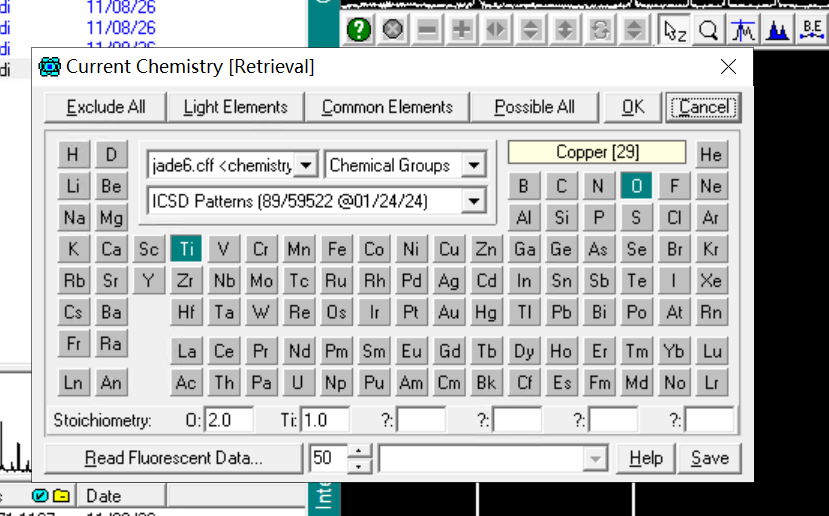
\includegraphics[width=\linewidth,height=4.8cm,keepaspectratio]{assets/jade/jade_01_pdf_search.png}
    \caption{按 Ti--O 化学式检索}
  \end{subfigure}\hfill
  \begin{subfigure}[t]{0.32\textwidth}
    \centering
    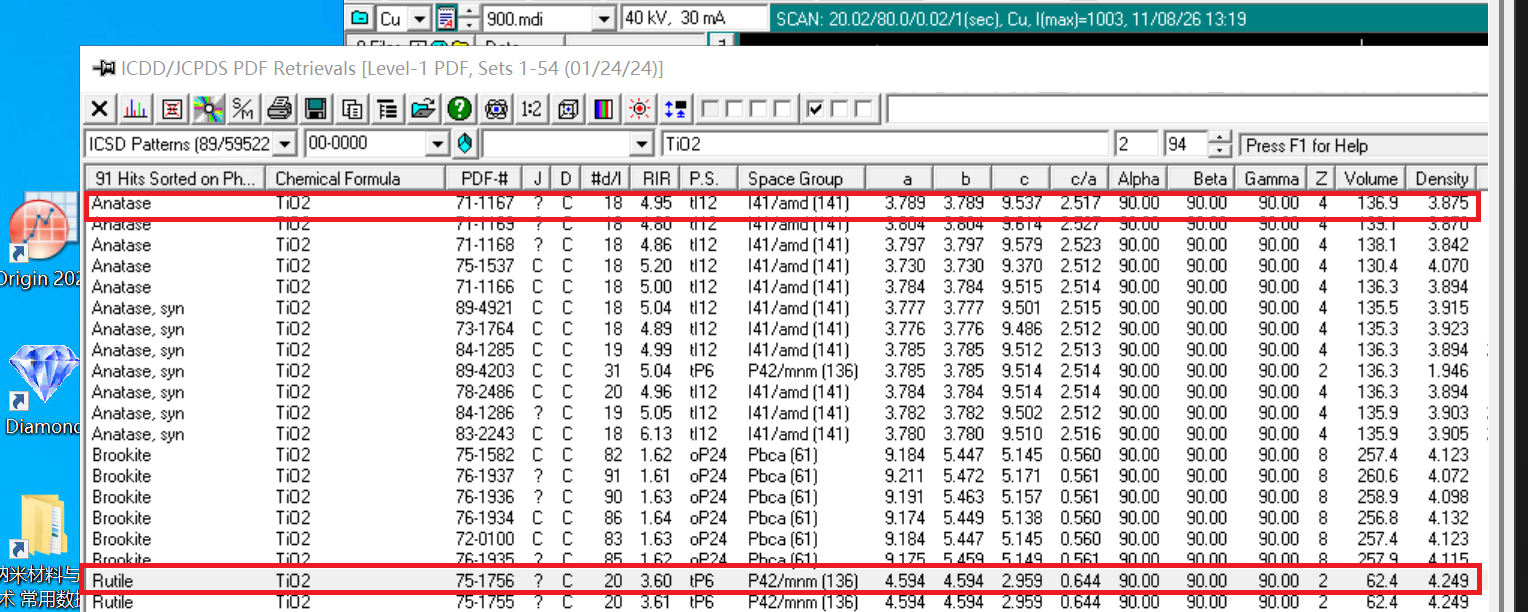
\includegraphics[width=\linewidth,height=4.8cm,keepaspectratio]{assets/jade/jade_02_pdf_data.png}
    \caption{锐钛矿 71-1167 / 金红石 75-1756}
  \end{subfigure}\hfill
  \begin{subfigure}[t]{0.32\textwidth}
    \centering
    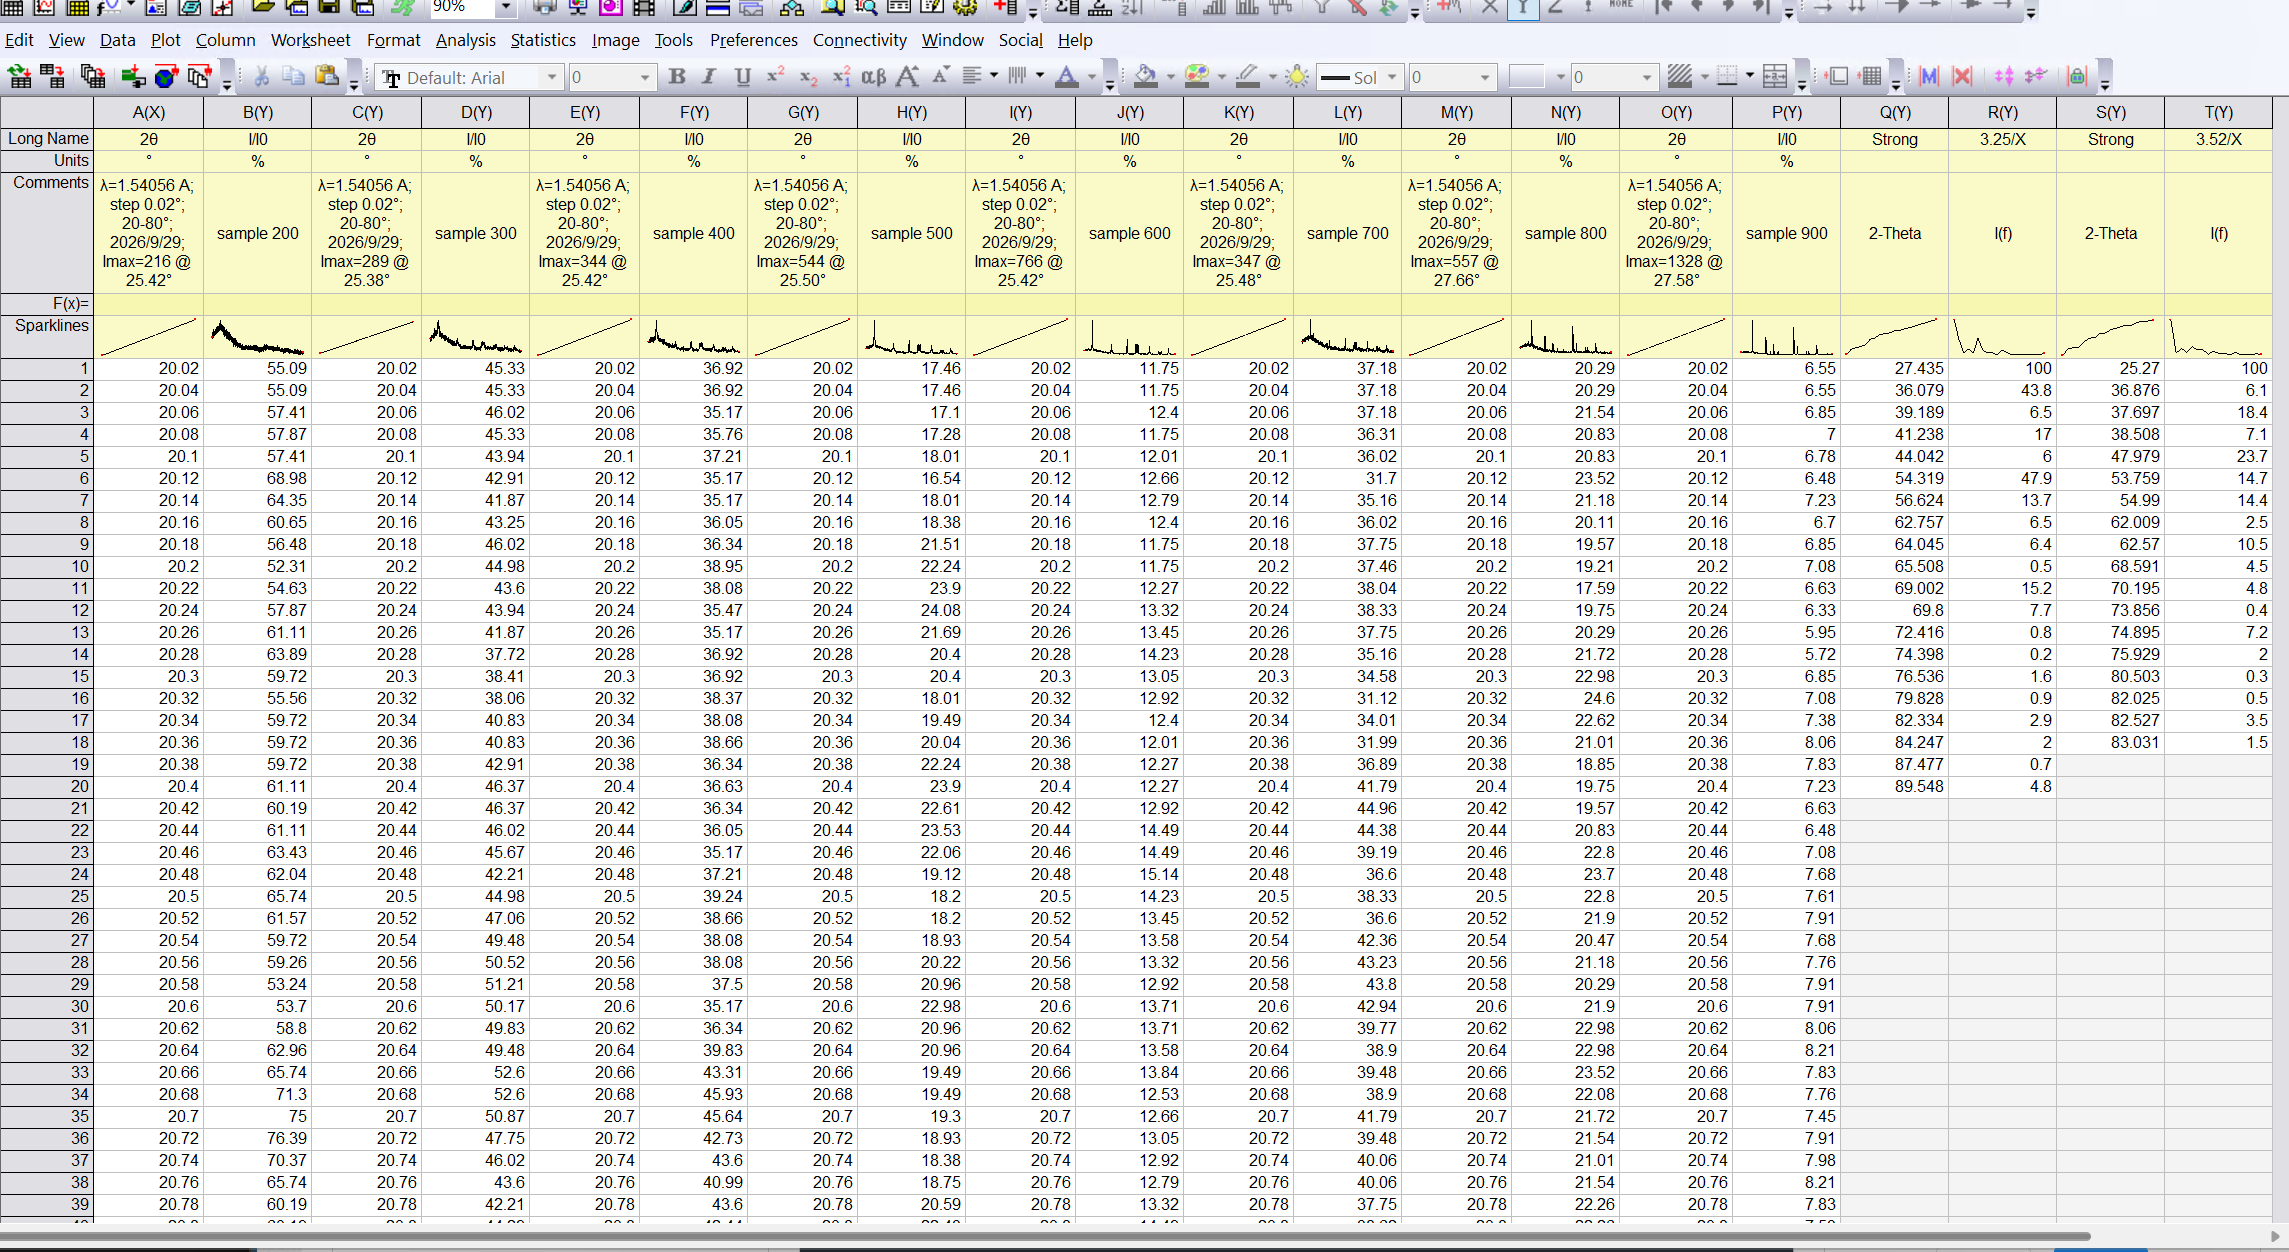
\includegraphics[width=\linewidth,height=4.8cm,keepaspectratio]{assets/jade/jade_03_columns.png}
    \caption{保留 $2\theta$ 与强度}
  \end{subfigure}
  \caption{Jade 中检索 PDF 卡片并整理数据。(a) 在 Current Chemistry 中选择 Ti、O，化学式 Ti1O2；(b) 检索结果中的锐钛矿 71-1167 与金红石 75-1756（红框）；(c) 把卡片数据复制到工作表，只保留 $2\theta$ 和强度两列。}
  \label{fig:jade}
\end{figure}

卡片数据往往有很多列（$d$ 值、相对强度、$hkl$ 等），画图只需要 $2\theta$ 和相对强度 $I/I_0$ 两列。把这两列复制到工作表右侧，删掉不需要的列，得到图~\ref{fig:jade}(c) 那样的总表；表~\ref{tab:pdf} 列出两张卡片的主要衍射线，可以逐峰对照。表中数据来自 Jade 检索到的 71-1167 / 75-1756。

\begin{table}[H]
  \centering
  \caption{Jade 检索到的锐钛矿 71-1167 与金红石 75-1756 主要衍射线}
  \label{tab:pdf}
  \small
  % 作业二 PDF 卡片数据（Jade 检索到的 71-1167 / 75-1756）
\begin{tabular}{@{}cccccc@{}}
\toprule
\multicolumn{3}{c}{锐钛矿 71-1167} & \multicolumn{3}{c}{金红石 75-1756} \\
\cmidrule(lr){1-3}\cmidrule(lr){4-6}
$2\theta$/$^\circ$ & $I/I_0$/\% & $hkl$ & $2\theta$/$^\circ$ & $I/I_0$/\% & $hkl$ \\
\midrule
25.28 & 100 & (101) & 27.45 & 100 & (110) \\
36.95 & 10 & (103) & 36.09 & 50 & (101) \\
37.80 & 20 & (004) & 39.19 & 8 & (200) \\
38.58 & 10 & (112) & 41.23 & 25 & (111) \\
48.05 & 35 & (200) & 44.05 & 10 & (210) \\
53.89 & 20 & (105) & 54.32 & 60 & (211) \\
55.06 & 20 & (211) & 56.64 & 20 & (220) \\
62.12 & 4 & (213) & 62.75 & 10 & (002) \\
62.69 & 14 & (204) & 64.04 & 10 & (310) \\
68.76 & 6 & (116) & 69.01 & 20 & (301) \\
70.31 & 6 & (220) & 69.79 & 12 & (112) \\
74.03 & 2 & (107) &  &  &  \\
75.03 & 10 & (215) &  &  &  \\
76.02 & 4 & (301) &  &  &  \\
\bottomrule
\end{tabular}

  \par\vspace{3pt}
  {\footnotesize 注：常用卡片 21-1272（锐钛矿）和 21-1276（金红石）的主峰位置与上表一致，弱峰强度在不同数据库版本中略有差别。}
\end{table}

\subsection{在 Origin 中画 PDF 卡片并叠加}

PDF 卡片的横坐标是 $2\theta$，纵坐标是相对强度，画出来是一组竖线（棒图），不是折线。绘制和叠加按 6 步进行，与截图一一对应。

\paragraph{步骤 1：选中 PDF 数据并 Stackplot}
在 Origin 中选中 PDF 卡片的 $2\theta$ 和强度列，先把 $2\theta$ Set As X，再执行 \texttt{Plot $\rightarrow$ Stackplot}，如图~\ref{fig:pdf-step1}。

\begin{figure}[H]
  \centering
  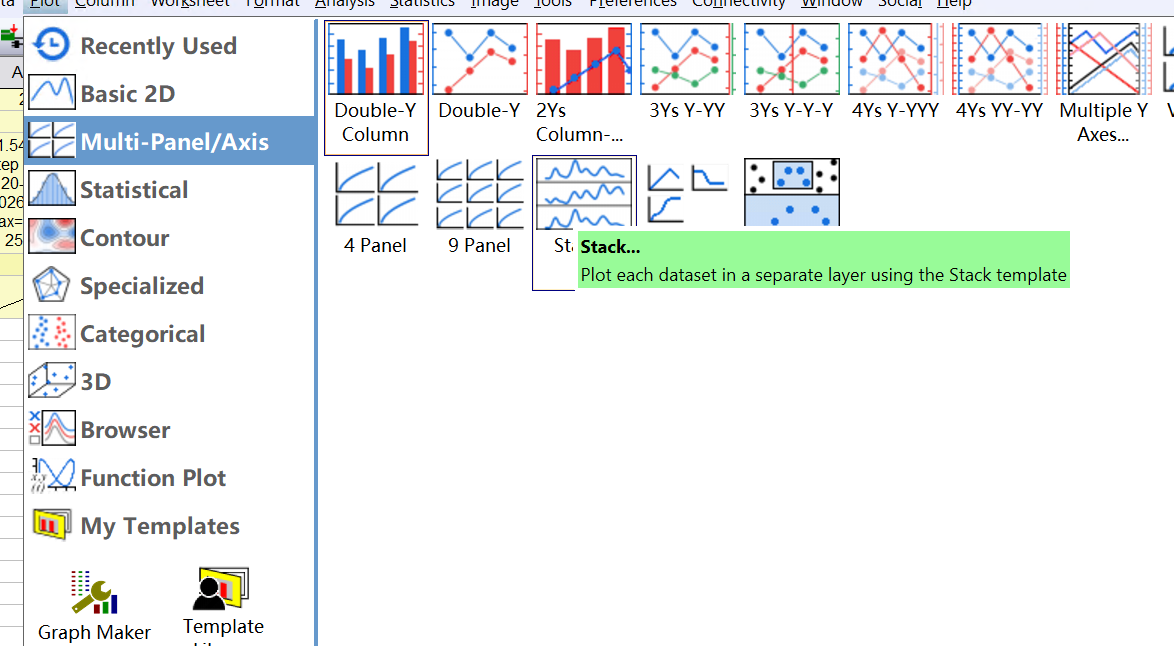
\includegraphics[width=\textwidth,height=6.5cm,keepaspectratio]{assets/origin/origin_04_pdf_stack.png}
  \caption{步骤 1：选中 PDF 卡片的 $2\theta$ 和强度列，Plot $\rightarrow$ Stackplot。}
  \label{fig:pdf-step1}
\end{figure}

\paragraph{步骤 2：Plot Type 选 Column}
弹出的 \texttt{Stack: plotstack} 对话框中，Plot Type 选 \texttt{Column}，Input 里确认是 \texttt{PDF\#71-1167} 的两列数据，点 OK 就得到一张只有竖线的卡片图，如图~\ref{fig:pdf-step2}。

\begin{figure}[H]
  \centering
  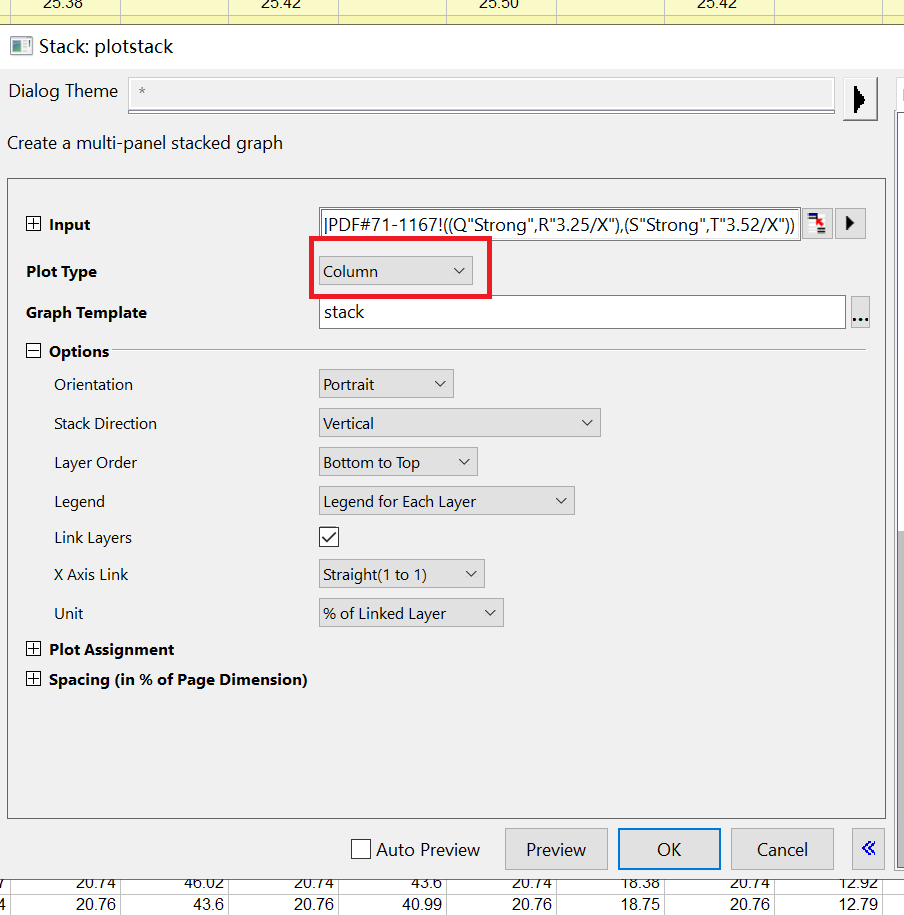
\includegraphics[width=\textwidth,height=6.5cm,keepaspectratio]{assets/origin/origin_05_column.png}
  \caption{步骤 2：Stack plot 对话框，Plot Type 选 Column。}
  \label{fig:pdf-step2}
\end{figure}

\paragraph{步骤 3：在 Layer2/Layer3 中放卡片}
图~\ref{fig:pdf-step3} 是 \texttt{Plot Details} 里的 Layer 结构：Layer1 是主图，Layer2 和 Layer3 分别放锐钛矿和金红石的卡片；Plot Type 选 \texttt{Column / Bar}，勾选 \texttt{Bar}，卡片就以柱状图显示。

\begin{figure}[H]
  \centering
  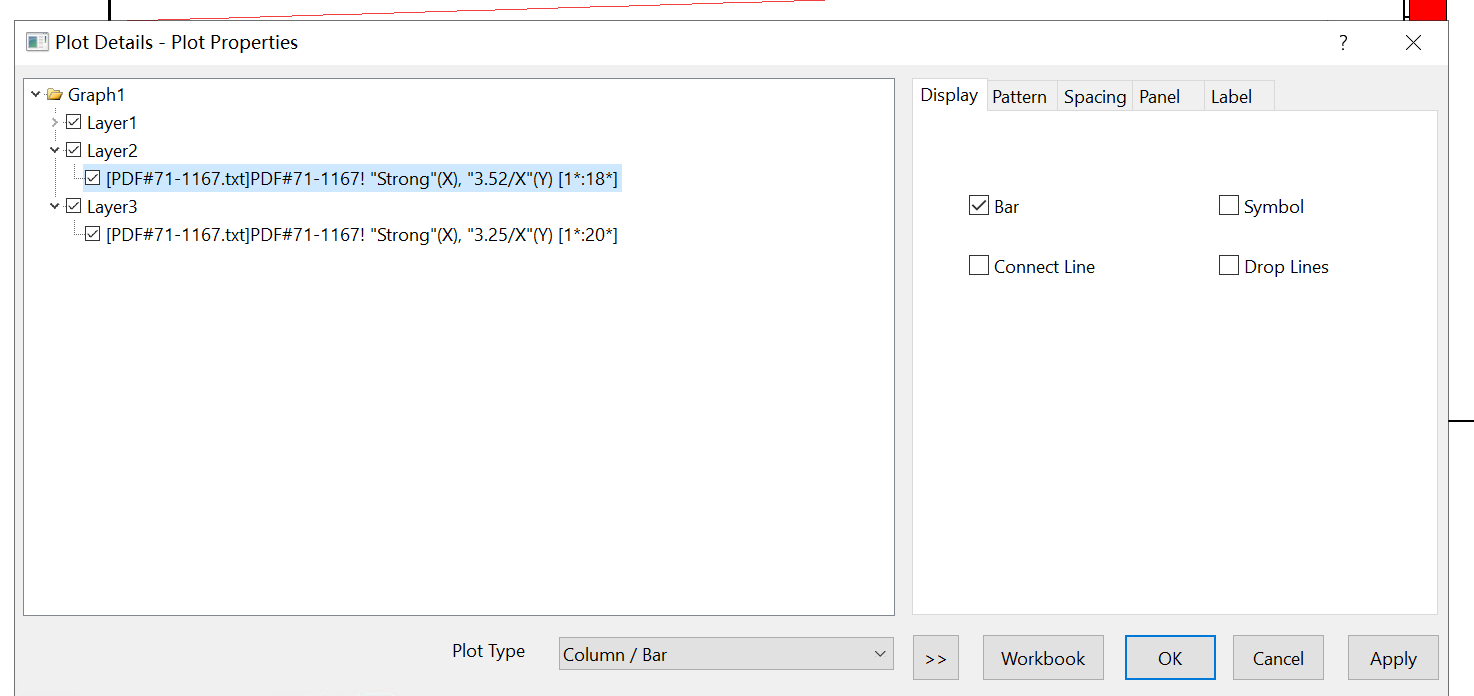
\includegraphics[width=\textwidth,height=6.5cm,keepaspectratio]{assets/origin/origin_06_layer.png}
  \caption{步骤 3：Plot Details 中 Layer2/Layer3 放卡片，勾选 Bar。}
  \label{fig:pdf-step3}
\end{figure}

\paragraph{步骤 4：导入 PDF 数据时选 Start New Columns}
导入 PDF 卡片数据时，第一个文件也要选 \texttt{Start New Columns}，否则卡片数据会覆盖主图数据，如图~\ref{fig:pdf-step4}。

\begin{figure}[H]
  \centering
  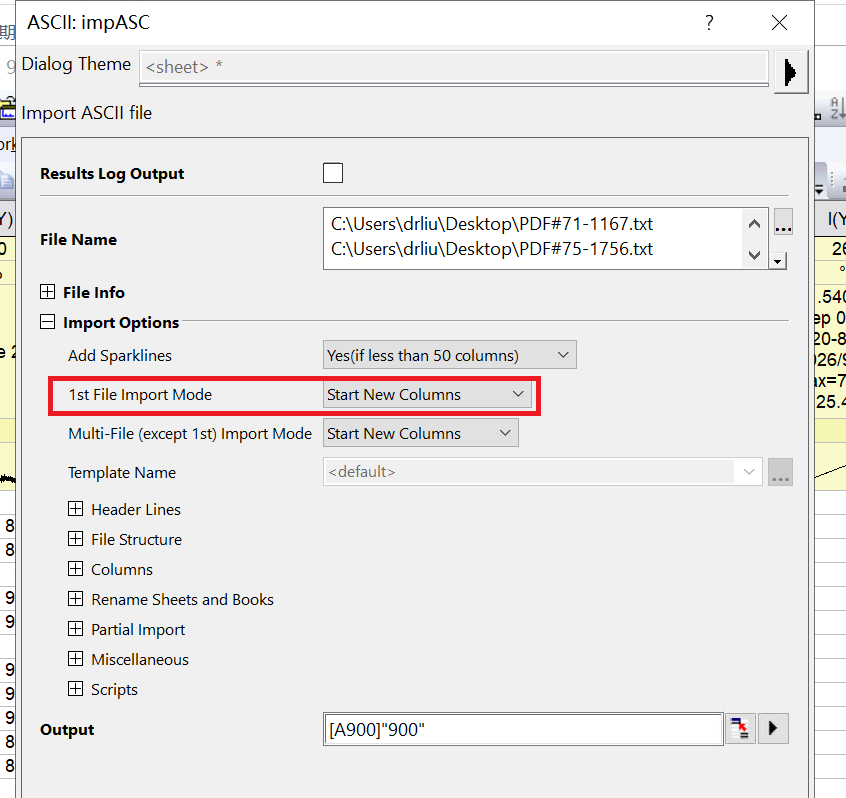
\includegraphics[width=\textwidth,height=6.5cm,keepaspectratio]{assets/origin/origin_pdf_import.png}
  \caption{步骤 4：导入 PDF 卡片数据时选 Start New Columns。}
  \label{fig:pdf-step4}
\end{figure}

\paragraph{步骤 5：设置卡片层的 X 轴}
卡片层的 X 轴必须和主图一致。图~\ref{fig:pdf-step5} 是 \texttt{X Axis - Layer 3} 对话框，把范围设成 20--80$^\circ$，再按需要调 Scale 和 Tick Labels。

\begin{figure}[H]
  \centering
  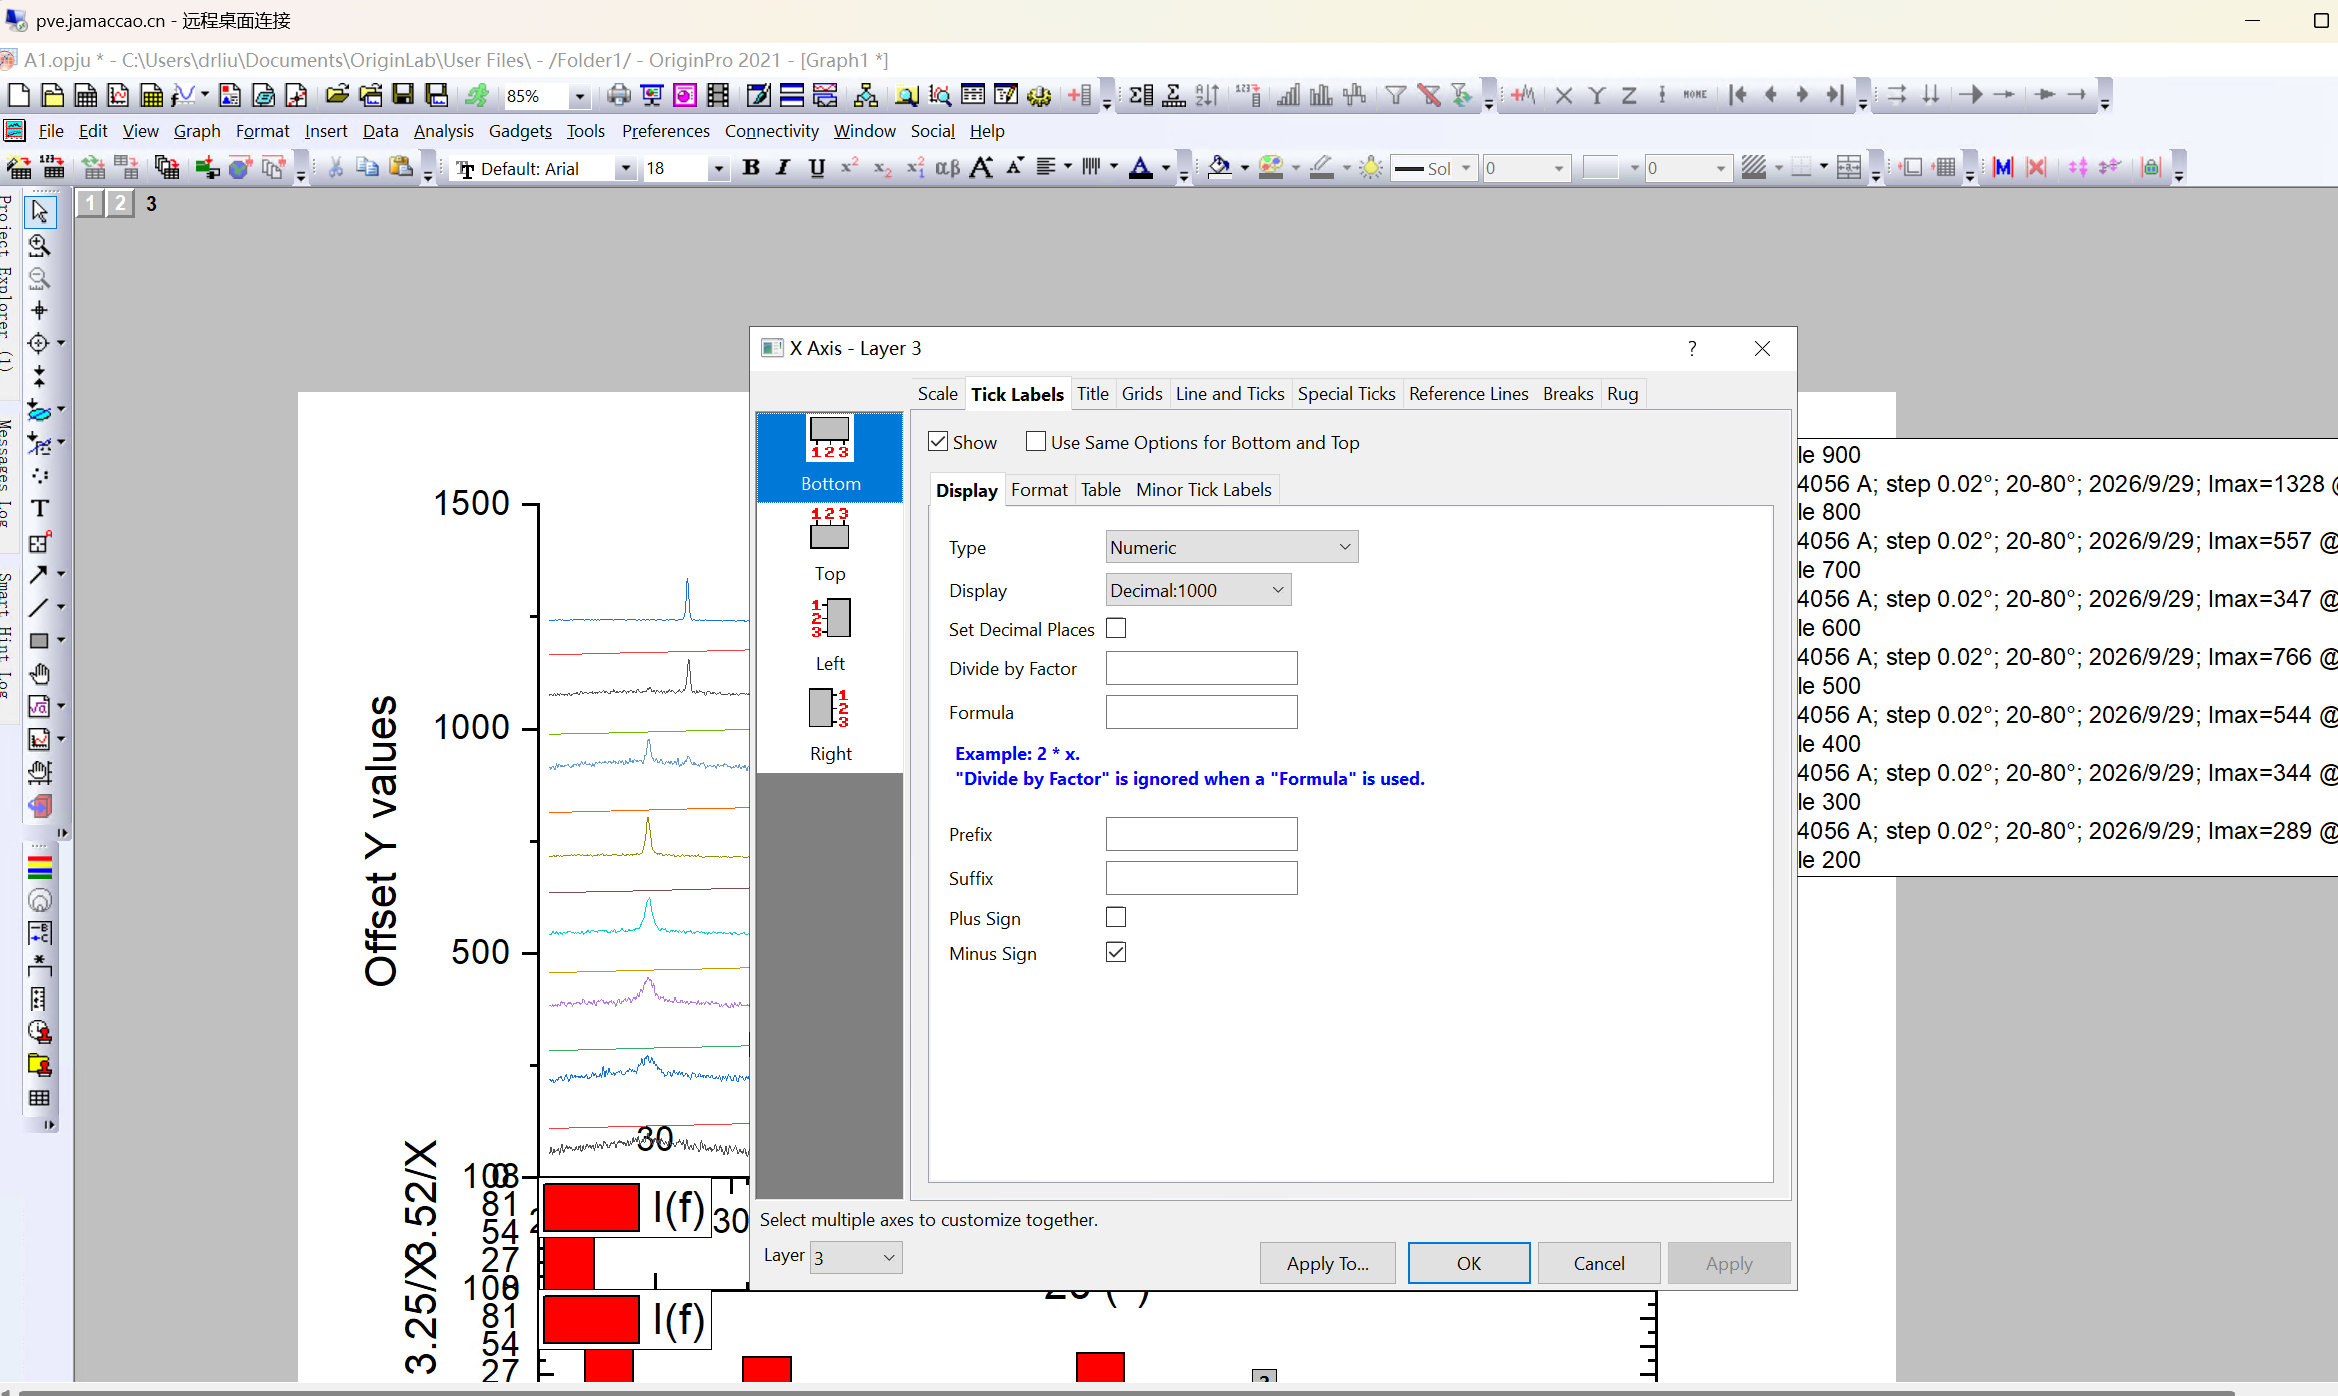
\includegraphics[width=\textwidth,height=6.5cm,keepaspectratio]{assets/origin/origin_axis_layer.png}
  \caption{步骤 5：X Axis - Layer 3 中设置卡片层范围/刻度。}
  \label{fig:pdf-step5}
\end{figure}

\paragraph{步骤 6：调整位置并得到最终结果}
卡片图作为新层贴到主图上之后，位置和大小要反复调：主图设为左 15、上 10、宽 70、高 60，卡片层高 10 左右；双击图像本体在 Size 选项卡里调位置和大小，双击边框在 Scale 和 Lines and Ticks 里调范围和刻度，Layer 选项卡调颜色。锐钛矿用绿色、金红石用红色，两套卡片放在主图下方两行，中间留一条细横线。结果见图~\ref{fig:pdf-step6}。

\begin{figure}[H]
  \centering
  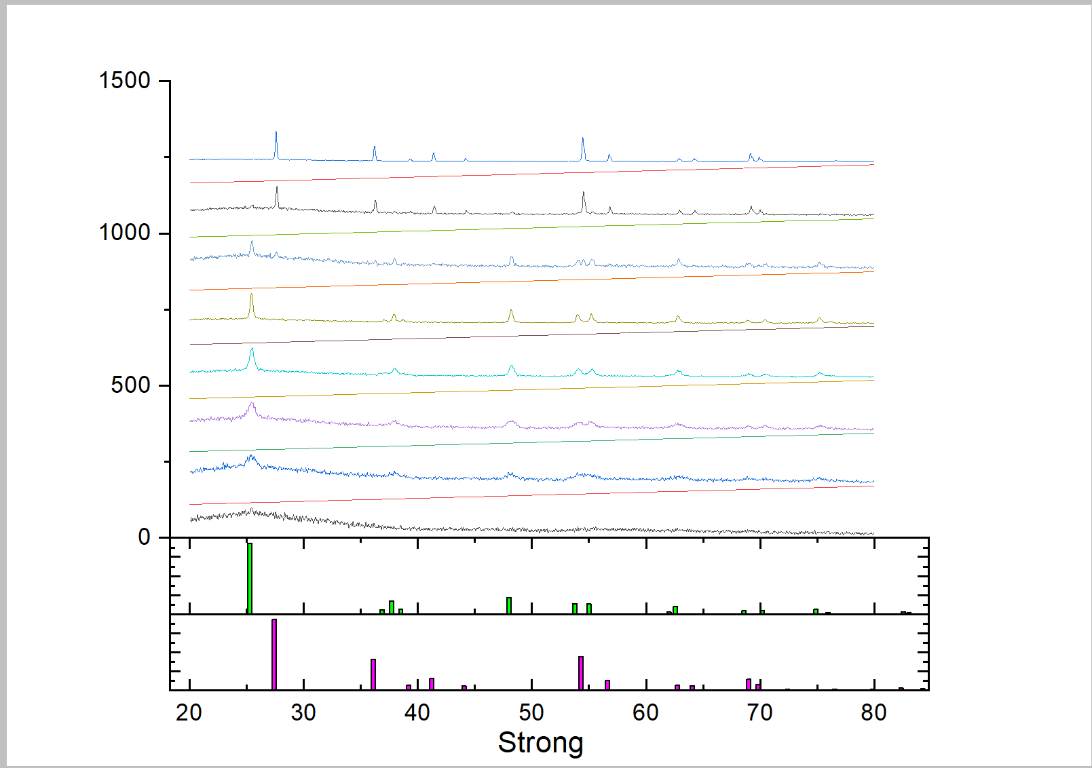
\includegraphics[width=\textwidth,height=6.5cm,keepaspectratio]{assets/origin/origin_07_final.png}
  \caption{步骤 6：Origin 中得到的最终结果（8 条曲线 + 两套卡片）。}
  \label{fig:pdf-step6}
\end{figure}

\subsection{最终多曲线图}

图~\ref{fig:xrd} 汇总了 8 组谱线和两套卡片。Origin 导出的原始图在缩放和图例上不够清楚，这张图改用 \pyB 从 \texttt{ready\_norm} 的数据重绘；曲线、卡片位置和偏移量与图~\ref{fig:pdf-step6} 一致，只调整了图例、刻度和局部放大。图 (a) 是 20--80$^\circ$ 的全谱，8 条曲线按温度从下到上偏移；图 (b) 是锐钛矿 71-1167 和金红石 75-1756 的标准棒图；图 (c) 是 23--30$^\circ$ 的局部放大，虚线标出 A(101) 和 R(110) 的卡片位置。

\begin{figure}[tbp]
  \centering
  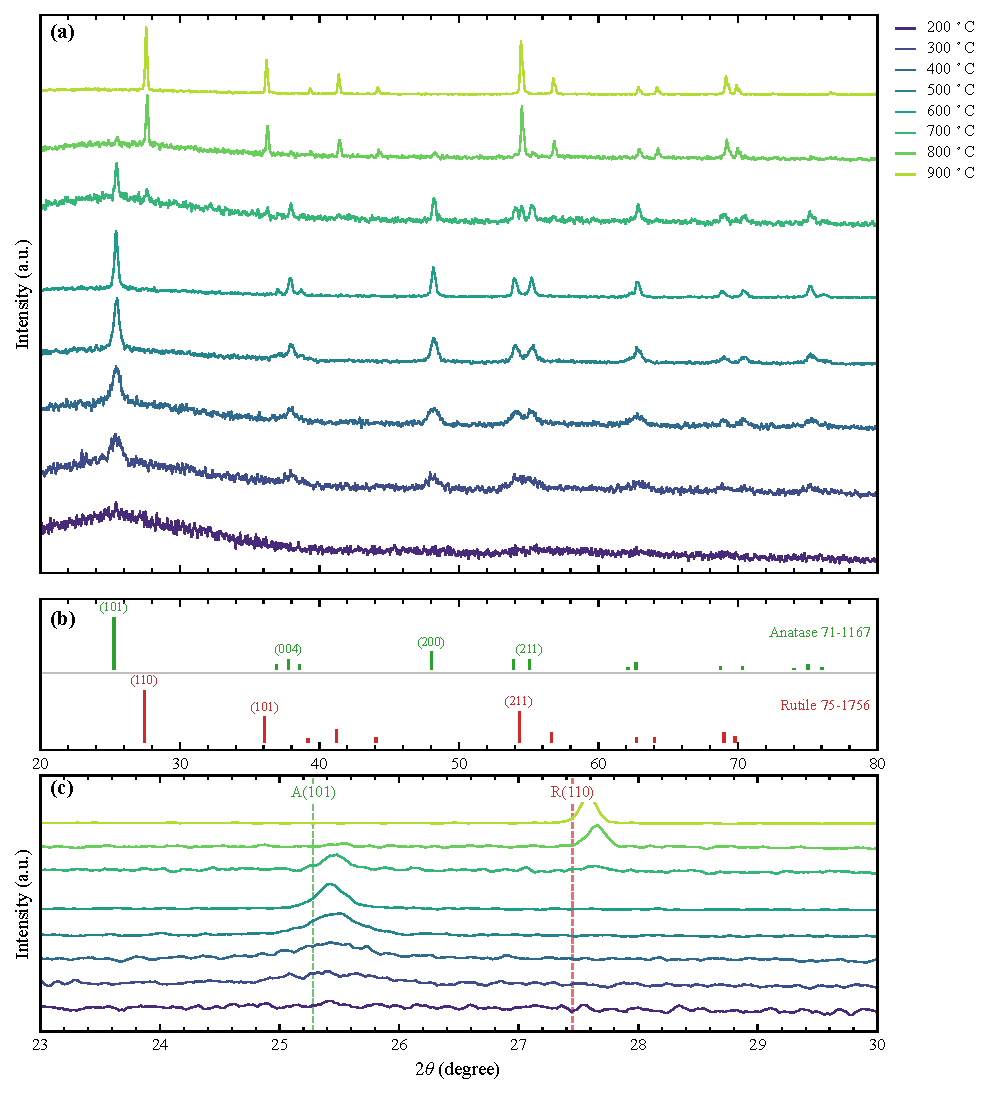
\includegraphics[width=0.95\textwidth]{assets/xrd/fig1_xrd_stack.pdf}
  \caption{200--900 $^\circ$C 系列 TiO$_2$ 样品的 XRD 多曲线图与 PDF 卡片。(a) 全谱，曲线经 \pyA 转换并各自归一化到最强峰，沿 Y 方向偏移；(b) 锐钛矿 71-1167（上）与金红石 75-1756（下）的标准棒图；(c) $2\theta=23^\circ$--$30^\circ$ 的局部放大，虚线为 A(101) 与 R(110) 的卡片位置。}
  \label{fig:xrd}
\end{figure}

\subsection{物相描述}

温度对物相的影响在图~\ref{fig:xrd} 上比较清楚。200 $^\circ$C 的谱线在 25.4$^\circ$ 附近只有一个很宽的包，背底从低角向高角缓慢下降，说明样品结晶度很低，只能看到一个宽化的锐钛矿 (101) 包络。300--600 $^\circ$C 的谱线已经能清楚地和锐钛矿卡片对上：25.4$^\circ$ 的 (101)、37.8$^\circ$ 的 (004)、48.0$^\circ$ 的 (200)、54.0$^\circ$ 的 (105) 和 55.1$^\circ$ 的 (211) 都能找到，其中 (101) 最强，和卡片的相对强度一致。700 $^\circ$C 的谱线在 27.6$^\circ$ 出现一个新峰，位置与金红石 (110) 对应；36.1$^\circ$ 附近也能看到金红石 (101) 的弱峰。800 $^\circ$C 的谱线中，金红石的 (110)、(101)、(211) 都很明显，同时还能看到锐钛矿 (101) 的残余；900 $^\circ$C 则只剩金红石的峰，锐钛矿的峰基本消失。

表~\ref{tab:phase} 按样品列出上面读到的特征峰。峰位从图上直接读取，误差约 ±0.1$^\circ$，只用来区分峰的归属。

\begin{table}[H]
  \centering
  \caption{由图~\ref{fig:xrd} 读出的主要物相与特征峰}
  \label{tab:phase}
  \small
  \begin{tabular}{@{}p{1.2cm}p{3.2cm}p{10.8cm}@{}}
    \toprule
    样品 & 主要物相 & 特征峰（$2\theta$/$^\circ$，$hkl$） \\
    \midrule
    200 & 低结晶度锐钛矿 & 25.4 (101)，宽包 \\
    300--600 & 锐钛矿 & 25.4 (101)、37.8 (004)、48.0 (200)、54.0 (105)、55.1 (211) \\
    700 & 锐钛矿 + 少量金红石 & 25.5 (101)、27.6 (110)、36.1 (101) \\
    800 & 锐钛矿 + 金红石 & 27.6 (110)、36.3 (101)、54.5 (211)；25.5 (101) 较弱 \\
    900 & 金红石 & 27.6 (110)、36.2 (101)、54.5 (211) \\
    \bottomrule
  \end{tabular}
  \par\vspace{3pt}
  {\footnotesize 注：峰位为图上直接读数，未做峰拟合。}
\end{table}
